\documentclass[svgnames]{article}
\usepackage{listings}


\lstset{language=C++,
                basicstyle=\tiny\ttfamily,
                keywordstyle=\color{blue}\ttfamily,
                stringstyle=\color{red}\ttfamily,
                commentstyle=\color{Green}\ttfamily,
                morecomment=[l][\color{magenta}]{\#}
}


\usepackage{tikz}
\usetikzlibrary{arrows,positioning, calc, backgrounds,shapes.misc}
\tikzstyle{vertex}=[draw,fill=black!15,circle,minimum size=18pt,inner sep=0pt]
\tikzstyle{relink} = [DarkCyan, dashed, ->, >=stealth, shorten >= 1pt]

\begin{document}
\section{Morris Inorder Tree Traversal}
\subsection{source code}

\begin{tikzpicture}[
% background grid/.style={draw, very thin,step=0.25cm}, show background grid
]
\node[above right, inner sep=0] {
\begin{lstlisting}

/* Find predecessor */
Node* find_inorder_predecessor(Node* curr)
{
  Node* predecessor=curr->left;
  while (predecessor->right != NULL && predecessor->right != curr) 
    predecessor=predecessor->right; 
    
    return predecessor;
}

/* Morris Inorder traversal */
void morris_inorder_traversal(Node* root) 
{ 
  Node *curr; 
  curr = root; 
  
  while (curr!=NULL) 
  { 
    /* if curr doesn't have left child */
    if (curr->left==NULL) 
    { 
      cout<<curr->data<<" "; 
      curr=curr->right; 
    } 
    else 
    { 
        /* finding inorder predecessor */
    Node* predecessor=find_inorder_predecessor(curr);
      
      /* Make curr as the right child of its inorder predecessor */
      if(predecessor->right==NULL) 
      { 
        predecessor->right=curr; 
        curr=curr->left; 
      } 
      else 
      { 
        predecessor->right=NULL; 
        cout<<curr->data<<" "; 
        curr=curr->right; 
      }
    }
  }
}

int main() 
{  
  Node* root = new_node(1); 
  root->left = new_node(2); 
  root->right = new_node(5); 
  root->left->left = new_node(3); 
  root->left->right = new_node(4);
 /* this input tree is shown in above figure */
  cout<<"\nMorris Inorder Traversal of the graph: ";
  morris_inorder_traversal(root);

  return 0; 
}

\end{lstlisting}
};

% \foreach \x in {0,0.5,...,9} 
% \draw[very thick, blue] (\x, -1pt) -- (\x, 1pt) node[below, font=\tiny\bfseries] {\x};

% \foreach \y in {0,0.25,...,12} 
% \draw[very thick, red] (-1pt, \y) -- (1pt, \y) node[left, font=\tiny\bfseries] {\y};


\node[coordinate](lr) at (0.65, 7.6) {};
\node[coordinate] (ur) at (3.15, 7.8) {};

\path let \p1=(lr), \p2=(ur) in  coordinate (ae) at (\x2, {(\y2-\y1)/2 + \y1});
\node[above right=0.1cm and 0.3cm of ae, font=\tiny\ttfamily, fill=green!20, inner sep=1pt, rounded corners=0.2ex] (ab) {iteration 3};

\path[red, dashed, ->] (ab.west) edge[bend right] (ae);
\fill[red, opacity=0.3, rounded corners=0.3ex] (lr)rectangle (ur);


\node[coordinate](lr) at (0.65, 7.4) {};
\node[coordinate] (ur) at (2.6, 7.56) {};

\path let \p1=(lr), \p2=(ur) in  coordinate (ae) at (\x2, {(\y2-\y1)/2 + \y1});
\node[below right=0.1cm and 0.3cm of ae, font=\tiny\ttfamily, fill=green!20, inner sep=1pt, rounded corners=0.2ex] (ab) {\textbf{curr} moves from iteration 3 to iteration 4};

\path[red, dashed, ->] (ab.west) edge[bend left] (ae);
\fill[red, opacity=0.3, rounded corners=0.3ex] (lr)rectangle (ur);




\node[coordinate](lr) at (0.85, 4.25) {};
\node[coordinate] (ur) at (3.6, 4.45) {};

\path let \p1=(lr), \p2=(ur) in  coordinate (ae) at (\x2, {(\y2-\y1)/2 + \y1});
\node[above right=0.1cm and 0.3cm of ae, font=\tiny\ttfamily, fill=green!20, inner sep=1pt, rounded corners=0.2ex] (ab) {remove iteration 4 link};

\path[red, dashed, ->] (ab.west) edge[bend right] (ae);
\fill[red, opacity=0.3, rounded corners=0.3ex] (lr)rectangle (ur);


\node[coordinate](lr) at (0.85, 3.8) {};
\node[coordinate] (ur) at (2.8, 4.0) {};

\path let \p1=(lr), \p2=(ur) in  coordinate (ae) at (\x2, {(\y2-\y1)/2 + \y1});
\node[below right=0.1cm and 0.3cm of ae, font=\tiny\ttfamily, fill=green!20, inner sep=1pt, rounded corners=0.2ex] (ab) {move curr to iteration 5};

\path[red, dashed, ->] (ab.west) edge[bend left] (ae);
\fill[red, opacity=0.3, rounded corners=0.3ex] (lr)rectangle (ur);


\end{tikzpicture}


\subsection{Input Tree}
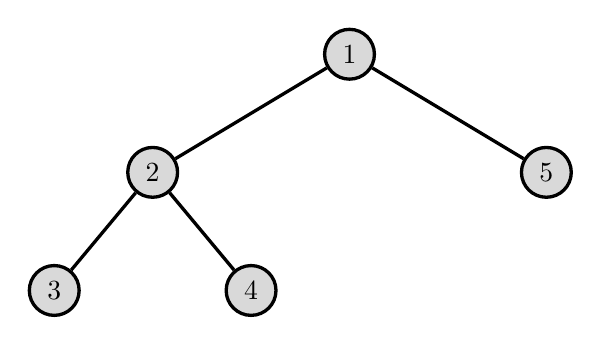
\begin{tikzpicture}[very thick, level/.style={sibling distance = 50mm/#1}]
  \node [vertex] (r){$1$}
  child {
    node [vertex] (a) {$2$}
    child 
    {
      node [vertex] {$3$}
    }
    child
    {
      node [vertex] {$4$}
    }
  }
  child {
    node [vertex] {$5$}
  };
\end{tikzpicture}

\subsection{Iterations}
\subsubsection{Iteration 1}

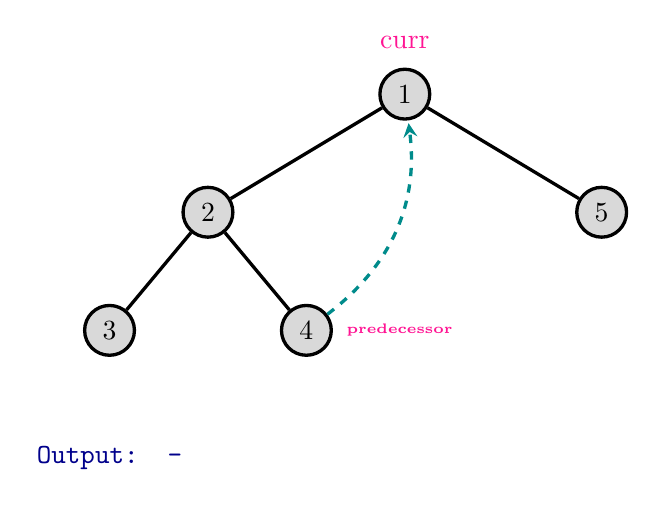
\begin{tikzpicture}[very thick, level/.style={sibling distance = 50mm/#1}]
  \node [vertex] (curr){$1$}
  child {
    node [vertex]  {$2$}
    child 
    {
      node [vertex] (ll){$3$}
    }
    child
    {
      node [vertex] (pre) {$4$}
    }
  }
  child {
    node [vertex] {$5$}
  };

\path[relink] (pre) edge[bend right] (curr);

\node [above=0.1cm of curr, text=DeepPink] {curr};
\node [right=1pt of pre, text=DeepPink, font=\tiny\bfseries] {predecessor};

\node [below=1cm of ll, font=\ttfamily\bfseries, text = DarkBlue] {Output: -};
\end{tikzpicture}


\subsubsection{iteration 2}
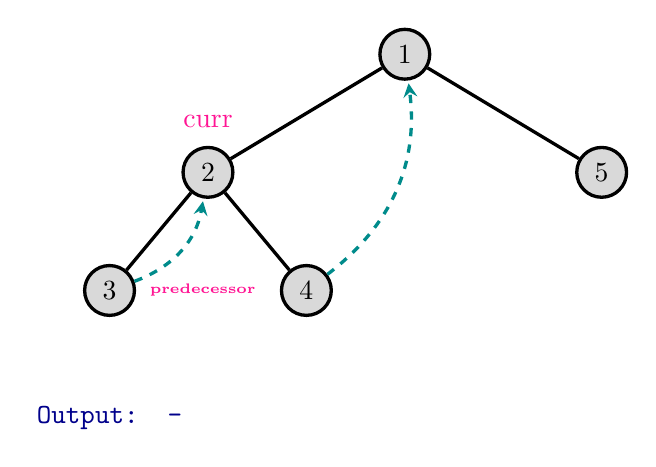
\begin{tikzpicture}[very thick, level/.style={sibling distance = 50mm/#1}]
  \node [vertex] (curr){$1$}
  child {
    node [vertex]  (curr2){$2$}
    child 
    {
      node [vertex] (pre2) {$3$}
    }
    child
    {
      node [vertex] (pre) {$4$}
    }
  }
  child {
    node [vertex] {$5$}
  };

\path[relink] (pre) edge[bend right] (curr);


\path[relink] (pre2) edge[bend right] (curr2);
\node [above=0.1cm of curr2, text=DeepPink] {curr};
\node [right=1pt of pre2, text=DeepPink, font=\tiny\bfseries] {predecessor};

\node [below=1cm of pre2, font=\ttfamily\bfseries, text = DarkBlue] {Output: -};

\end{tikzpicture}


\subsubsection{iteration 3}
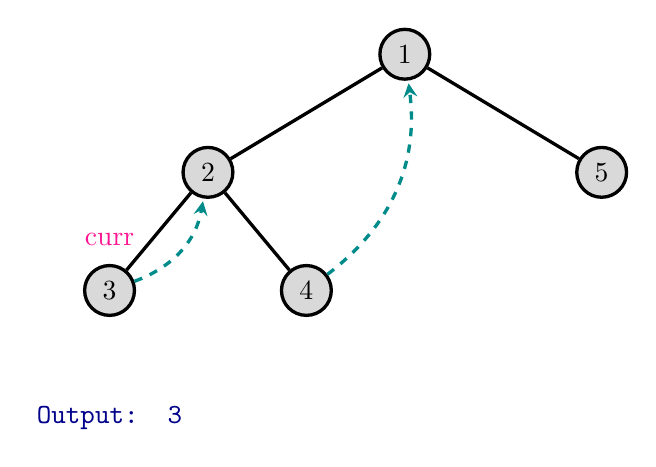
\begin{tikzpicture}[very thick, level/.style={sibling distance = 50mm/#1}]
  \node [vertex] (curr){$1$}
  child {
    node [vertex]  (curr2){$2$}
    child 
    {
      node [vertex] (pre2) {$3$}
    }
    child
    {
      node [vertex] (pre) {$4$}
    }
  }
  child {
    node [vertex] {$5$}
  };

\path[relink] (pre) edge[bend right] (curr);


\path[relink] (pre2) edge[bend right] (curr2);

\node [above=0.1cm of pre2, text=DeepPink] {curr};
% \node [right=1pt of pre2, text=DeepPink, font=\tiny\bfseries] {predecessor};

\node [below=1cm of pre2, font=\ttfamily\bfseries, text = DarkBlue] {Output: 3};
\end{tikzpicture}



\subsubsection{iteration 4}
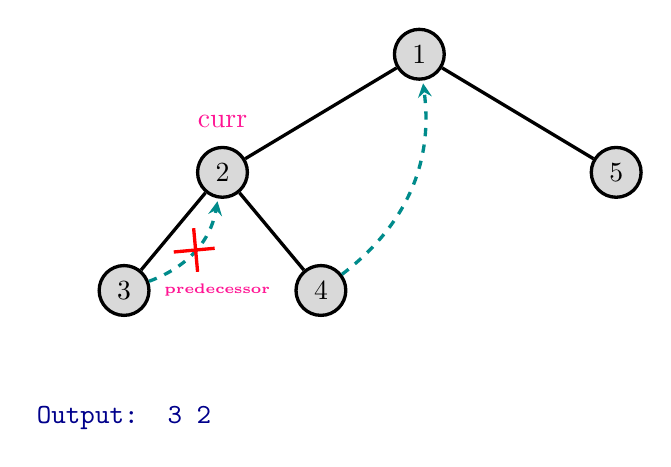
\begin{tikzpicture}[very thick, level/.style={sibling distance = 50mm/#1}]
  \node [vertex] (curr){$1$}
  child {
    node [vertex]  (curr2){$2$}
    child 
    {
      node [vertex] (pre2) {$3$}
    }
    child
    {
      node [vertex] (pre) {$4$}
    }
  }
  child {
    node [vertex] {$5$}
  };

\path[relink] (pre) edge[bend right] (curr);


\path[relink] (pre2) edge[bend right] node[sloped,minimum height=10pt, minimum width=10pt, inner sep=0, cross out,draw=red, solid] {} (curr2);

\node [above=0.1cm of curr2, text=DeepPink] {curr};
\node [right=1pt of pre2, text=DeepPink, font=\tiny\bfseries] {predecessor};

\node [below=1cm of pre2, font=\ttfamily\bfseries, text = DarkBlue] {Output: 3 2};

\end{tikzpicture}


\subsubsection{iteration 5}
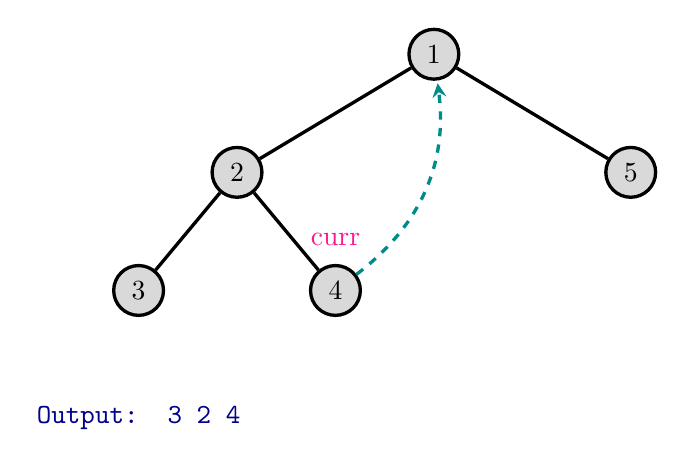
\begin{tikzpicture}[very thick, level/.style={sibling distance = 50mm/#1}]
  \node [vertex] (curr){$1$}
  child {
    node [vertex]  (curr2){$2$}
    child 
    {
      node [vertex] (pre2) {$3$}
    }
    child
    {
      node [vertex] (pre) {$4$}
    }
  }
  child {
    node [vertex] {$5$}
  };

\path[relink] (pre) edge[bend right] (curr);


% \path[relink] (pre2) edge[bend right] node[sloped,minimum height=10pt, minimum width=10pt, inner sep=0, cross out,draw=red, solid] {} (curr2);

\node [above=0.1cm of pre, text=DeepPink] {curr};
% \node [right=1pt of pre2, text=DeepPink, font=\tiny\bfseries] {predecessor};

\node [below=1cm of pre2, font=\ttfamily\bfseries, text = DarkBlue] {Output: 3 2 4};

\end{tikzpicture}


\subsubsection{iteration 6}
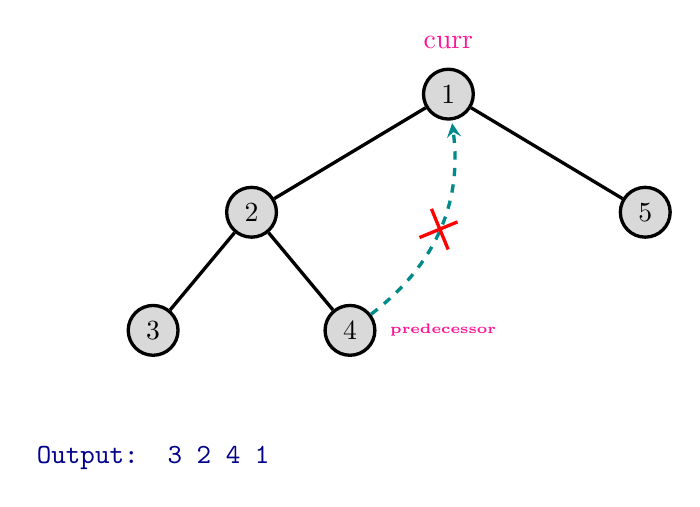
\begin{tikzpicture}[very thick, level/.style={sibling distance = 50mm/#1}]
  \node [vertex] (curr){$1$}
  child {
    node [vertex]  (curr2){$2$}
    child 
    {
      node [vertex] (pre2) {$3$}
    }
    child
    {
      node [vertex] (pre) {$4$}
    }
  }
  child {
    node [vertex] {$5$}
  };

\path[relink] (pre) edge[bend right] node[sloped,minimum height=10pt, minimum width=10pt, inner sep=0, cross out,draw=red, solid] {} (curr);


% \path[relink] (pre2) edge[bend right] node[sloped,minimum height=10pt, minimum width=10pt, inner sep=0, cross out,draw=red, solid] {} (curr2);

\node [above=0.1cm of curr, text=DeepPink] {curr};
\node [right=1pt of pre, text=DeepPink, font=\tiny\bfseries] {predecessor};

\node [below=1cm of pre2, font=\ttfamily\bfseries, text = DarkBlue] {Output: 3 2 4 1};

\end{tikzpicture}



\subsubsection{iteration 7}
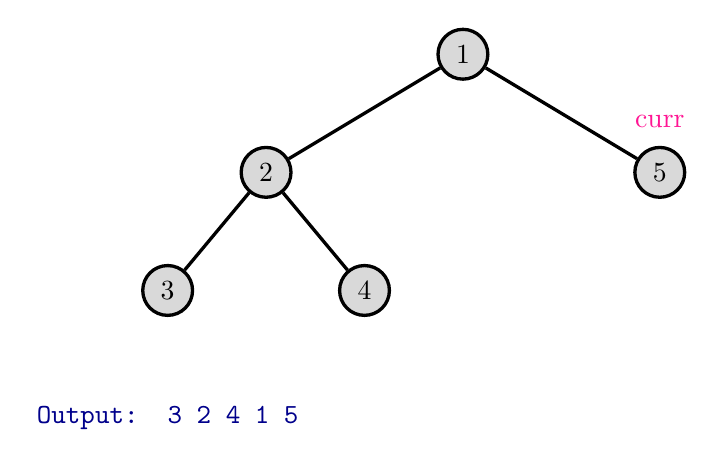
\begin{tikzpicture}[very thick, level/.style={sibling distance = 50mm/#1}]
  \node [vertex] (curr){$1$}
  child {
    node [vertex]  (curr2){$2$}
    child 
    {
      node [vertex] (pre2) {$3$}
    }
    child
    {
      node [vertex] (pre) {$4$}
    }
  }
  child {
    node [vertex] (curr3){$5$}
  };

% \path[relink] (pre) edge[bend right] node[sloped,minimum height=10pt, minimum width=10pt, inner sep=0, cross out,draw=red, solid] {} (curr);


% \path[relink] (pre2) edge[bend right] node[sloped,minimum height=10pt, minimum width=10pt, inner sep=0, cross out,draw=red, solid] {} (curr2);

\node [above=0.1cm of curr3, text=DeepPink] {curr};
% \node [right=1pt of pre, text=DeepPink, font=\tiny\bfseries] {predecessor};

\node [below=1cm of pre2, font=\ttfamily\bfseries, text = DarkBlue] {Output: 3 2 4 1 5};

\end{tikzpicture}


\end{document}